\section{Appendix}

\subsection{Daily kilometers average}
(on average, less than 5 trip per day)
\begin{figure}[h!]
    \centering
    \subfloat{
        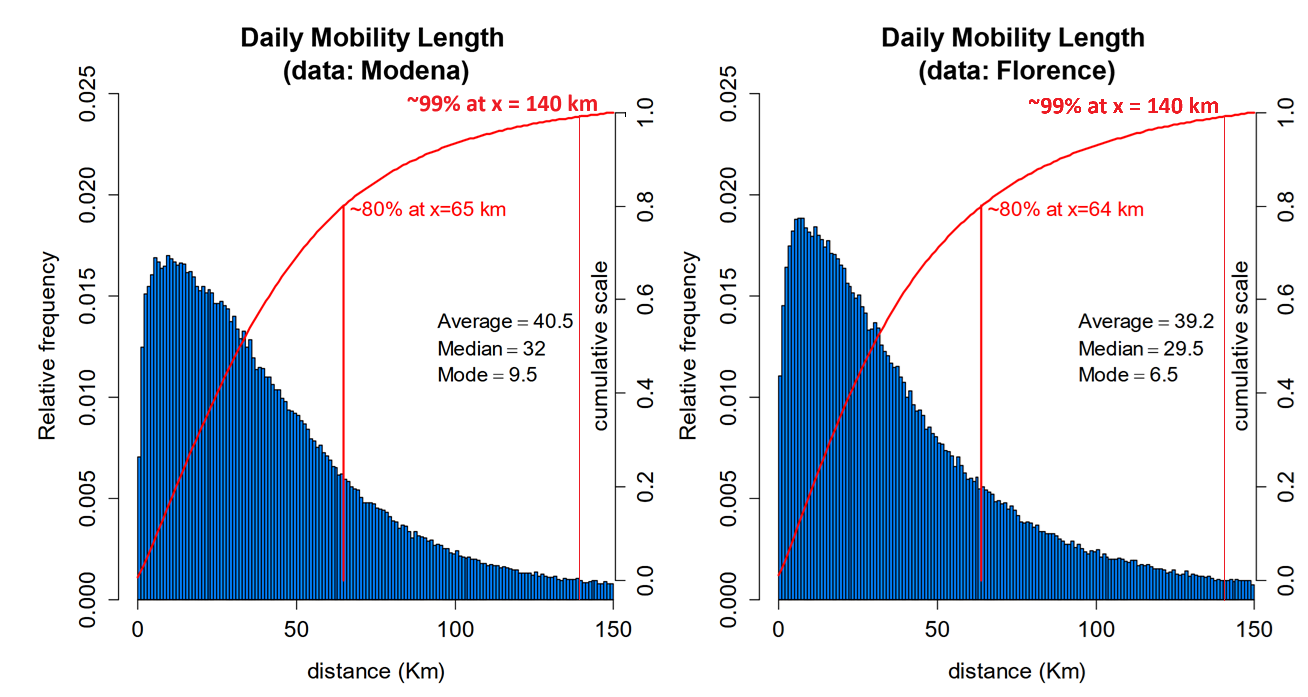
\includegraphics[width=0.97\linewidth]{Figures/ch2_DailyLenghtFrequencyPlot.png}
        \label{fig:daily-length}
    }
    \hfill
    \caption{Relative frequency (bar) and cumulative (red, solid) distributions of daily mobility distance (from Donati 2015\cite{donati_individual_2015})}
    \label{fig:daily-lenght-travel}
\end{figure}

\newpage 

\subsection{logbook}

\begin{itemize}[leftmargin=1.5cm,label={}]
    \item[\textbf{2025-02-20}] Creation of this report, rough layout of the idea in chapter
    
    \item[\textbf{2025-02-25}] Longitudinal kinematic model, research about markov modelling and cycle
    
    \item[\textbf{2025-02-26}] dynamic simulation creation, implemented a basic simulation in pybullet with keybaord navigation and parametric surface + wheel rolling down
    
    \item[\textbf{2025-02-27}] refining efficiency to take into account whole cycle, reading paper
    
    \item[\textbf{2025-02-28}] Writing Idea about improving efficiency trough identified parameters

    \item[\textbf{2025-03-04}] Adding graph about car occupancy and real world driving needs + reading paper

    \item[\textbf{2025-03-06}] Brainstorming kinematic, reading PHd thesis on narrow track

    \item[\textbf{2025-03-09}] URDF is a PAIN to implement to due lack of tool, trying to define a kinematic model in python

    \item[\textbf{2025-03-11}] reworking part of chapter 2

    \item[\textbf{2025-03-17}] reading paper about cars and bike and limiting factor to adoption

    \item[\textbf{2025-03-18}] keep reading paper, also about narrow track vehicle

    \item[\textbf{2025-03-20}] trying to structure what I learned from the papers

    \item[\textbf{2025-03-21}] defining the know unknown about car adoption factor (human side)

    \item[\textbf{2025-03-24}] Clarifying the project goal 

    \item[\textbf{2025-03-27}] draw figure, added citation

    \item[\textbf{2025-03-28}] Manual definition is an epic failure... Two way (createMultiBody -> Works but hard to read), Create body and add constraint don't work (rotation constraint crash the simulation.)

    \item[\textbf{2025-04-09}] Realized that createMultibody is more stable but has a "ghost" friction problem, Might as well use URDF then.

    \item[\textbf{2025-04-10}] learning URDF and how the origin is defined, 

    \item[\textbf{2025-05-25}] redefined most variant as URDF and how to simulate them. Need spend time to implement basic controller like PID to show steady state stability and control margin

    \item[\textbf{2025-05-28}] Meeting, dry run presentation  and shown current status.

    \item[\textbf{2025-05-31}] Report restructuring, writing

    \item[\textbf{2025-06-02}] Chapter 4, 5, 6 writing
\end{itemize}
